\section*{Teoretická část}
Tranzistor je jedna ze základních elektronických součástek.
Skládá se ze dvou P-N přechodů.
V této úloze budeme měřit vlastnosti křemíkového tranzistoru BD 139 typu NPN při zapojení se společným emitorem.

Pro měření vstupní charakteristiky tranzistor zapojíme podle schematu na obrázku \ref{obr:schemavstup}.
Nastavíme požadovaný odpor $R$ a při nulovém napětí na bázi nastavíme napětí na kolektoru $U_{CE} = \SI{5}{\volt}$ a dále ho neměníme.


Pro měření výstupní charakteristiky zapojíme tranzistor podle schematu na obrázku \ref{obr:schemavystup}.

Pro měření činitele proudového zesílení necháme tranzistor v zapojení podle schematu na obrázku \ref{obr:schemavystup}.


\begin{figure}[htbp]
\centering
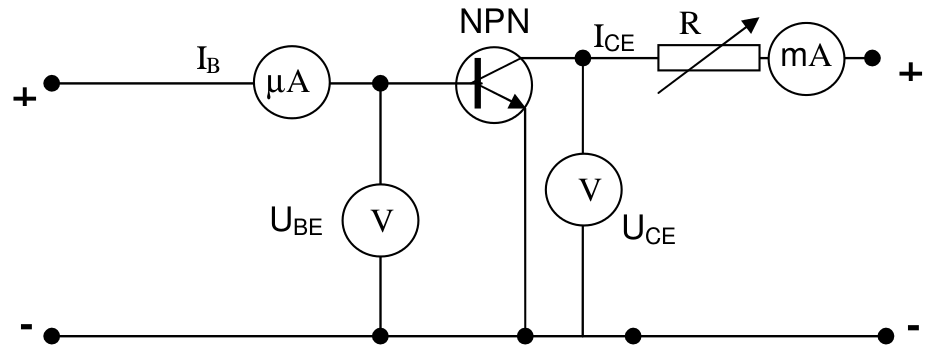
\includegraphics[width=\textwidth-2cm]{graficos/vstup}
\caption{Zapojení pro měření vstupní charakteristiky\cite{skripta}}
\label{obr:schemavstup}
\end{figure}

\begin{figure}[htbp]
\centering
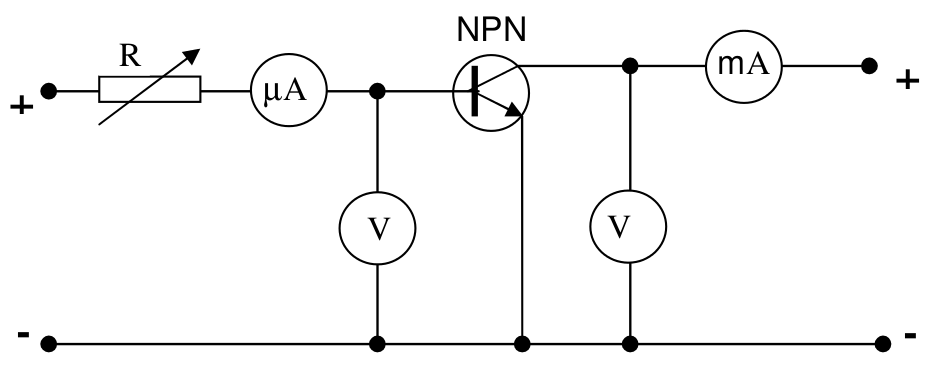
\includegraphics[width=\textwidth-2cm]{graficos/vystup}
\caption{Zapojení pro měření výstupní charakteristiky\cite{skripta}}
\label{obr:schemavystup}
\end{figure}